\item A bola $B$ tem massa de \SI{10}{\kilogram} e está fixada à ponta de uma barra cuja massa pode ser desprezada. Se
o eixo é submetido a um torque $M=(2\,t^{2} + 4)\SI{}{\newton\meter}$, onde t está em segundos, determine a velocidade
da bola quanto $t=\SI{2}{\second}$. A bola tem uma velocidade $v=\SI{2}{\meter/\second}$ quanto $t=0$.

\import{sections/answers/}{answer-13}

\vspace{-1.7cm}
\begin{flushright}
	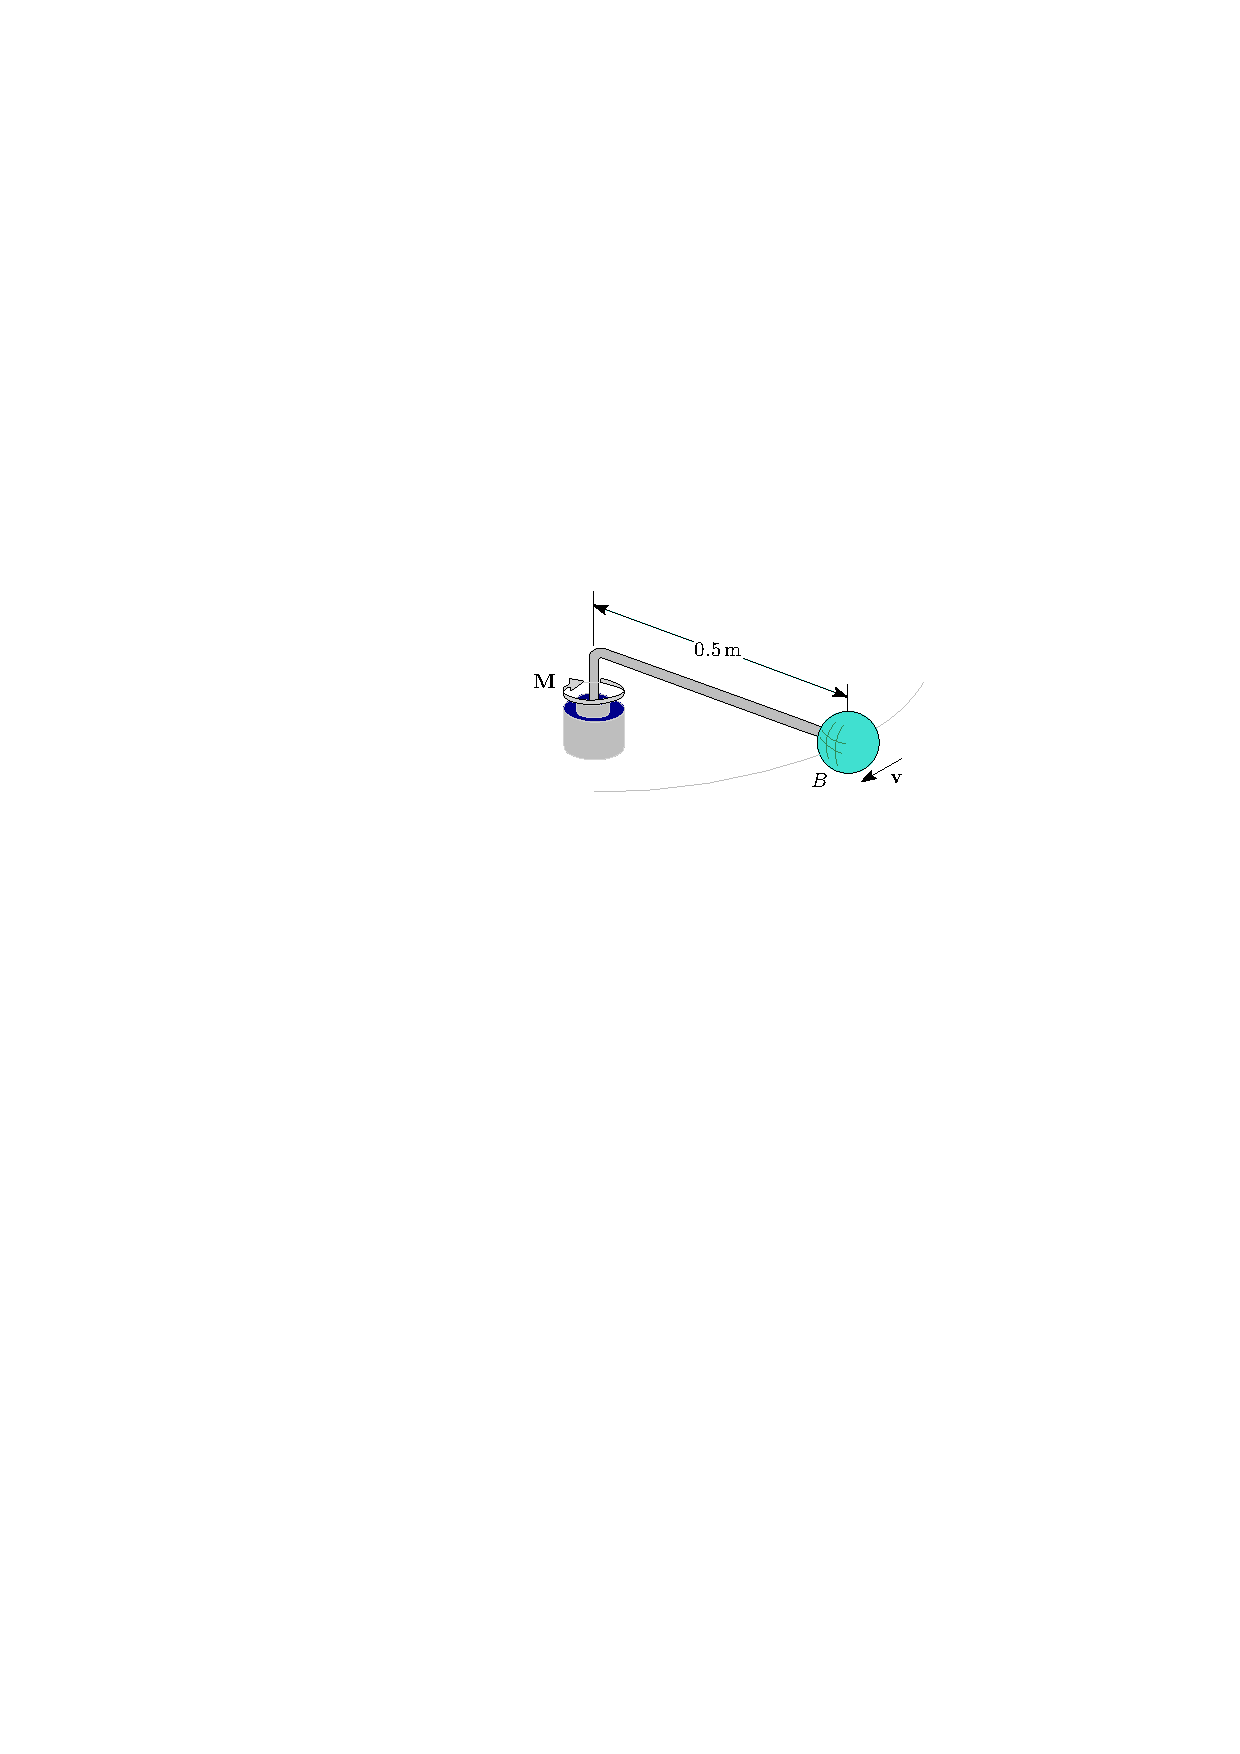
\includegraphics[scale=1.3]{images/draw_9}
\end{flushright}